\chapter{Software}
Dieser Abschnitt wird auf die Implementation der Software eingegangen und es werden die wichtigsten Schritte behandelt, die für die Datenversendung und Verarbeitung entscheidend waren.
\section{Prozessor Setup}

Das Setup beider Prozessor Boards ist aus Vereinheitlichung identisch, bis auf das Abrufen der spezifischen IMUs wurden alle Programmierabschnitte gleich geschrieben. 
\\
Dabei wurden folgende Bibliotheken ausgesucht:
\begin{itemize}
    \item \textbf{Adafruit MPU6050} von Adafruit Industries, erlaubt das lesen von Daten aus dem MPU-6050\parencite{web:Adafruit}
    \item \textbf{DFRobot BMI160} von DFRobot Shanghai, erlaubt das lesen von Daten aus dem BMI160 \parencite{web:DFRobot}
    \item \textbf{MPU9250} aus der Arduino Bibliothek, erlaubt das lesen von Daten aus dem MPU-9250
    \item \textbf{UDPConnection} eine selbst entwickelte, ausschließlich für dieses Projekt implementierte Bibliothek, erlaubt UDP Pakete oder Daten Serial zu versenden 
\end{itemize}

Das \lstinline{Setup()} für die Initialisierung des ESP32 beginnt mit dem überprüfen der Verbindungsart, ob es sich um eine direkte Verbindung über den USB Port oder das Netzwerk handelt. Dieses entscheidet ob der Prozessor die Daten über den Serial Port oder die WiFi Verbindung, als UDP Paket versendet und erlaubt somit, unabhängig von Verbindung, Zugang auf die Daten zu gewähren. Das UDP Protokoll ist ein Kommunikationsprotokoll, welches eine Verbindung zwischen Anwendungen im Internet erstellt.
Durch das senden der Daten ohne jeglichen empfangenden Host ist dieser eine schnelle und zeitkritische Kommunikation, welche für kleinere Pakete die versendet werden sehr vorteilhaft sind, da diese ohne Zeitverzögerung das Ziel erreichen können. Die Pakete werden mit definierten Header versendet, den Ursprungs Port, den Ziel Port, die Paket Länge und einer Prüfsumme, wobei jedes Feld 2 Byte groß ist. 
\\
\\
In Kapitel \ref{MUX} wurde auf die limitierten Zugänge der $I^{2}C$ Ports eingegangen, dabei wurde der \textit{TCA9548A} als Erweiterung dieser hinzugefügt. Die Funktion \lstinline{tcaselect(uint8_t i)} erlaubt es uns somit die Ports direkt auf dem \textit{TCA9548A} aufzurufen, jedoch kann sich dieses als sehr ungeeignet wegen der statischen Struktur für die Architektur auswirken und für zukünftige Weiterentwicklung problematisch stellen.
Dafür wurde die Funktion \textit{identifyIMU()} hinzugefügt, welche alle Ports des MUX auf verfügbare Adressen prüft. Beim auffinden einer Verbindung, abhängig der Adresse wird der Port aufgerufen und entsprechend des verfügbaren IMU Modells initialisiert. Durch die zwei weitern Ports ist es möglich weiter Sensoren zu Datenerfassung anzuschließen, ohne die Limitierung des ESP32 in kauf zu nehmen.
\begin{lstlisting}
void identifyIMU(){
  for (uint8_t t=0; t<8; t++) {
      tcaselect(t);
      Serial.print("TCA Port #"); Serial.println(t);

      for (uint8_t addr = 0; addr<=127; addr++) {
        if (addr == TCAADDR) continue;

        Wire.beginTransmission(addr);
        if (!Wire.endTransmission()) {
          Serial.print("Found I2C 0x");  Serial.println(addr,HEX);
          if(addr != 0xC){
          initMPU(t);
}}}}}
\end{lstlisting}

Um die Kommunikation zwischen Host-PC und den beiden Handschuhen ohne Unterscheidung zu gewähren, versenden beide die gleiche Datenstruktur, das erlaubt uns eine identische Datenübertragung, ohne auf das Sensormodell zu achten. 
\\
\\
Die abgelesenen Daten werden kontinuierlich in der \lstinline{loop()} Anweisung ausgegeben, dabei wird sicher gegangen das jeder Port überprüft wird, falls noch weitere IMUs angebracht werden. Während des Initialisierungs Prozess werden die Ports, welche mit einem Sensor belegt waren innerhalb eines Arrays auf ein Wert gesetzt, hierfür steht eins für einen Finger oder drei für die Mittelhand. 
\begin{lstlisting}
void loop(){
  for(uint8_t i=0; i<8; i++){
        if(foundIMU[i] == 1 && readMPUFinger(i, buffer, seq)){
            udp.sendImuData(fingers ,buffer, i);
            seq = (seq + 1) % 255; 
        }else if(foundIMU[i] == 3 && readMPUCore(i, buffer, seq)){
            udp.sendImuData(palm, buffer, i);
            seq = (seq + 1) % 255; 
}}}
\end{lstlisting}
Mit der \lstinline{readMPU} Funktion werden die Daten innerhalb des Parameters \textit{buffer} gefüllt und über die UDPConnection Bibliothek auf dem Serial Port geschrieben oder mit einer UDP Datei verschickt.


\section{ROS System}
Um diese Daten in ablesbare Messungen zu wandeln, werden sie über das ROS System verarbeitet. ROS steht für Robotic Operating System, dieses besitzt verschiedene Bibliotheken und Funktionen mit denen es möglich ist Programme zu entwickeln die für die Robotik bestimmt sind. 
Sie können Daten übernehmen, die aus unterschiedlichen Sensoren gewonnen werden und konvertieren diese um in geordneten Daten, beispielsweise für die Orientierung, Analyse und Erfassung der Umgebung. 
\\
\\
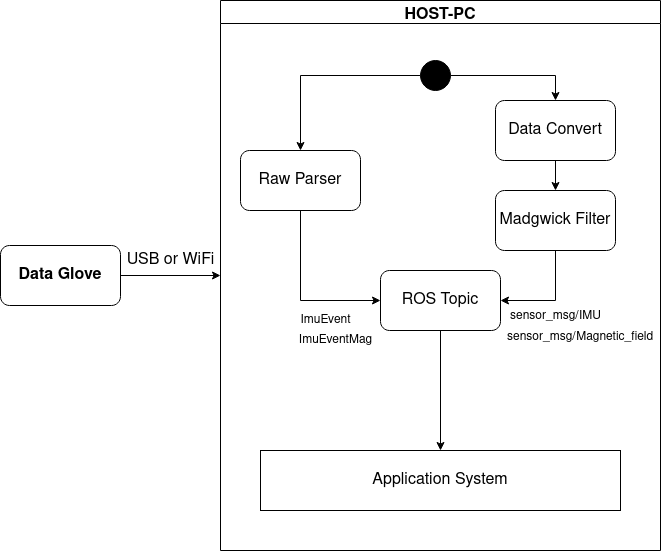
\includegraphics[width=0.7\columnwidth]{Bachelorarbeit/images/Host-Architektur.drawio.png}
\\
\\
Um die versendeten Werte gebräuchlich zu formatieren, können diese zuerst in der folgenden Datenstruktur um konvertiert werden. 
\begin{lstlisting}[label=lst:structure]
IMU{
std_msgs/Header header
geometry_msgs/Quaternion orientation
float64[9] orientation_covariance
geometry_msgs/Vector3 angular_velocity
float64[9] angular_velocity_covariance
geometry_msgs/Vector3 linear_acceleration
float64[9] linear_acceleration_covariance
}
\end{lstlisting}
Diese Konvertierung wird in der \lstinline{convertPublisher} Klasse bewerkstelligt, hierbei werden alle Finger einem Topic zugeteilt. Ein Topic ist eine benannte Aufgabe, über die Nodes Nachrichten austauschen können. Diese Nodes besitzen Publisher oder Subscriber, die ihre Informationen an andere weitergeben oder empfangen können. Wird ein Node ausgeführt können die Topics über diverse Mittel abgelesen oder gespeichert werden.
\\
In den Folgenden Messungen wurden die Handschuh ohne Bewegung und ohne die Position festzulegen gemessen. 

\begin{figure}[h]
	\centering
    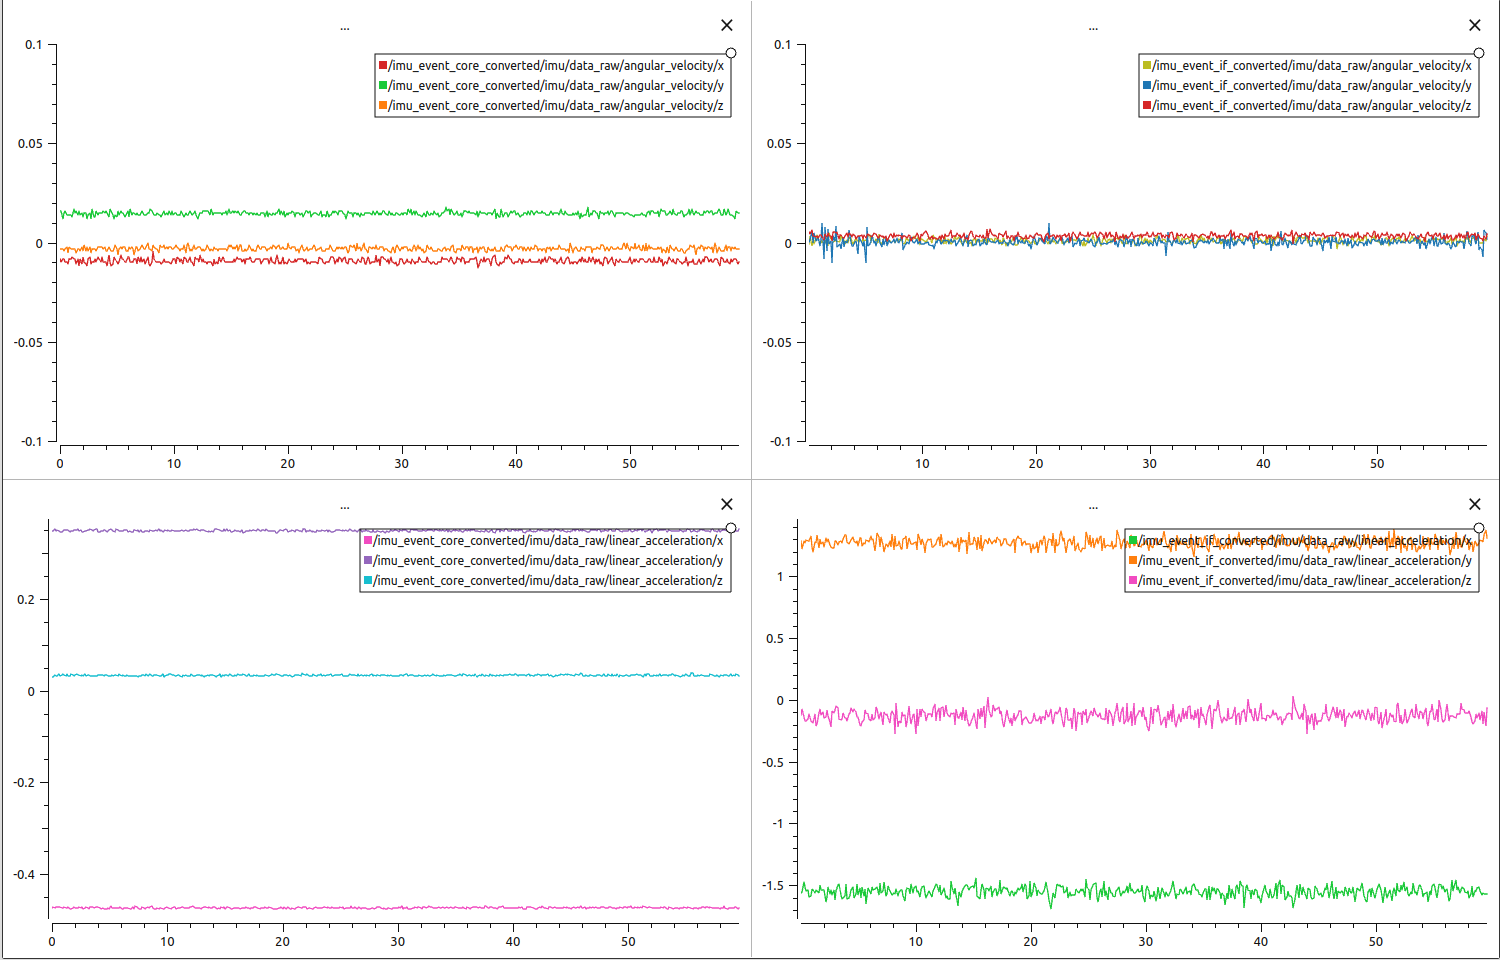
\includegraphics[width=1\columnwidth]{Bachelorarbeit/images/160-9250-RawData.png}
    \caption{Rohdaten des MPU-9250(links) und dem BMI160(rechts)}
    \label{fig:RawData160}
\end{figure}
Die Datenqualität des BMI160 Handschuh ist qualitativ Gut, es ist erkenntlich dass die Frequenz auf dem Handschuh gering ist. Durch Messungen der Datenrate wurde ermittelt das der BMI160 mit lediglich $8 Hz$ arbeitet, welches für das ermessen von Handbewegung nachteilig ist. 
\newpage
\begin{figure}[h]
	\centering
    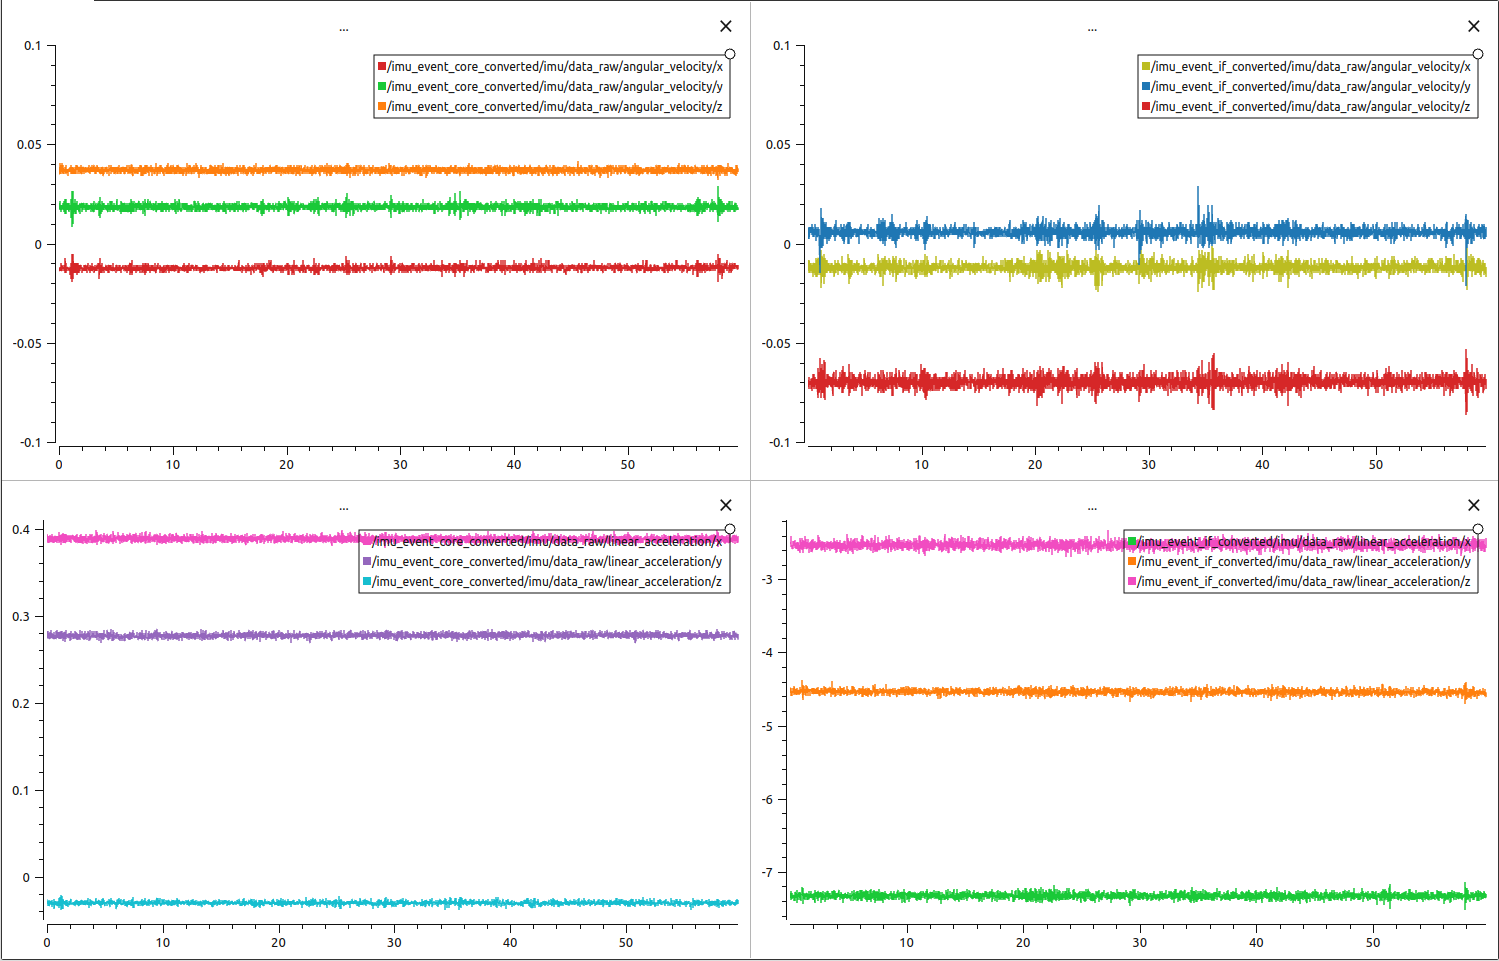
\includegraphics[width=1\columnwidth]{Bachelorarbeit/images/6050-9250RawData.png}
    \caption{Rohdaten des MPU-9250(links) und dem MPU-6050(rechts)}
    \label{fig:RawData6050}
\end{figure}
Der MPU-6050 Handschuh besitzt durch seine stärkere Leistung eine höhere Frequenz von $80 Hz$, das 10-fache des BMI160. Die Gravitationswerte für den MPU-6050 werden auf die Beschleunigung noch eingewirkt, dass hat die Konsequenz der verschobenen Werte.

Alle drei IMUs versenden lediglich nur die Beschleunigung und die Winkelgeschwindigkeit, bis auf den MPU-9250, der auch die Kompassdaten misst. Eines der Ziele für den Datenhandschuh war es das aufzeichnen der menschlichen Handbewegung, dafür wird die Orientierungen der Sensoren benötigt um die relative Position zu bestimmen. Zur Lösung dieses Problems wurde der Madgwick Filter verwendet. Der Madgwick Filter \parencite{Madgwick} fusioniert die Winkelgeschwindigkeit mit der Beschleunigung, optional auch den Kompass, um aus diesen Werten die Orientierung zu errechnen.
\\
Der Madgwick Filter ist ein Filteralgorithmus, welcher von Sebastian Madgwick entwickelt wurde. Für die Bestimmung der Orientierung gibt es zwei Möglichkeiten. 
Die Bestimmung der Orientierung nur mit der Winkelgeschwindigkeit ist ausführbar, jedoch für die präzise Ermittelung wird die Ausgangsorientierung benötigt, da sonst lediglich eine relative Orientierung zum Raum errechnet wird. Mit Hilfe der Beschleunigung, bzws. dem Magnetfeld wird das Gravitationsfeld oder auch das Magnetfeld der Erde bestimmt. Über diesen Vorgang kann die absolute Orientierung gemessen werden.
\\
Um den Madgwick Filter einzusetzen verwendet ROS das \lstinline{imu_filter_madgwick} Paket. Die verschiedenen Parameter die das Paket verwendet, werden über die ROS APIs aufgerufen. Sie können verwendet werden um den Gravitationsvektor zu entfernen, das Verstärken des Filters \lstinline{gain} mit dem höhere Werte zu einer schnelleren Konvergenz bestimmt werden, jedoch auch größerem Rauschen. Um die Parameter für die Finger zu definieren, so dass diese auch einzeln Topics zugehören, wird alles über eine launch Datei ausgeführt.
\\
\begin{lstlisting}
<node pkg="imusensor" type="convertPublisher.py" 
    name="convertedIMUData"/>

<node pkg="imu_filter_madgwick" type="imu_filter_node" 
    name="dataglove_filter_imu_{imuID}" output="screen">
    <param name="world_frame" value="enu"/>
    <param name="fixed_frame" value="world"/>
    <param name="use_mag"     value="false" />
    <param name="publish_tf"  value="true" />
    <param name="reverse_tf"  value="false" />
    <param name="constant_dt" value="0.0" />
    <param name="orientation_stddev" value="0.8"/>
    <param name="remove_gravity_vector" value="true"/>
    <!-- Parameter for the BMI Glove
    <param name="gain" value="1.0" />
    <param name="gain" value="0.0" />
    -->
    <!-- Parameter for the MPU
    <param name="gain" value="1.0" />
    <param name="gain" value="0.0" />
    -->
    <param name="gain" value="0.3" />
    <param name="zeta" value="0.1" />
    <remap from="/imu/mag" to="/imu_event_{imuID}_converted_mag/imu/mag" />
    <remap from="imu/data_raw" to="/imu_event_{imuID}_converted/imu/data_raw"/>
    <remap from="imu/data" to="/imu_event_{imuID}_converted/imu/data_fused"/>
</node>
\end{lstlisting}
Zu Beginn muss der Publisher starten, dabei werden die Datenprotokolle über 
\\
den \lstinline{convertPublisher.py} empfangen, in die zugehörige Datenstruktur\ref{lst:structure} konvertiert und publiziert. Dann muss man die Parameter, die in der Launch Datei gesetzt wurden, auf den jeweiligen Sensor anpassen. \newpage
Für den MPU-6050 ist die lineare Beschleunigung noch ungenau, da die Erdanziehungskraft auf die Sensoren einwirkt.

\begin{figure}[h]
	\centering
    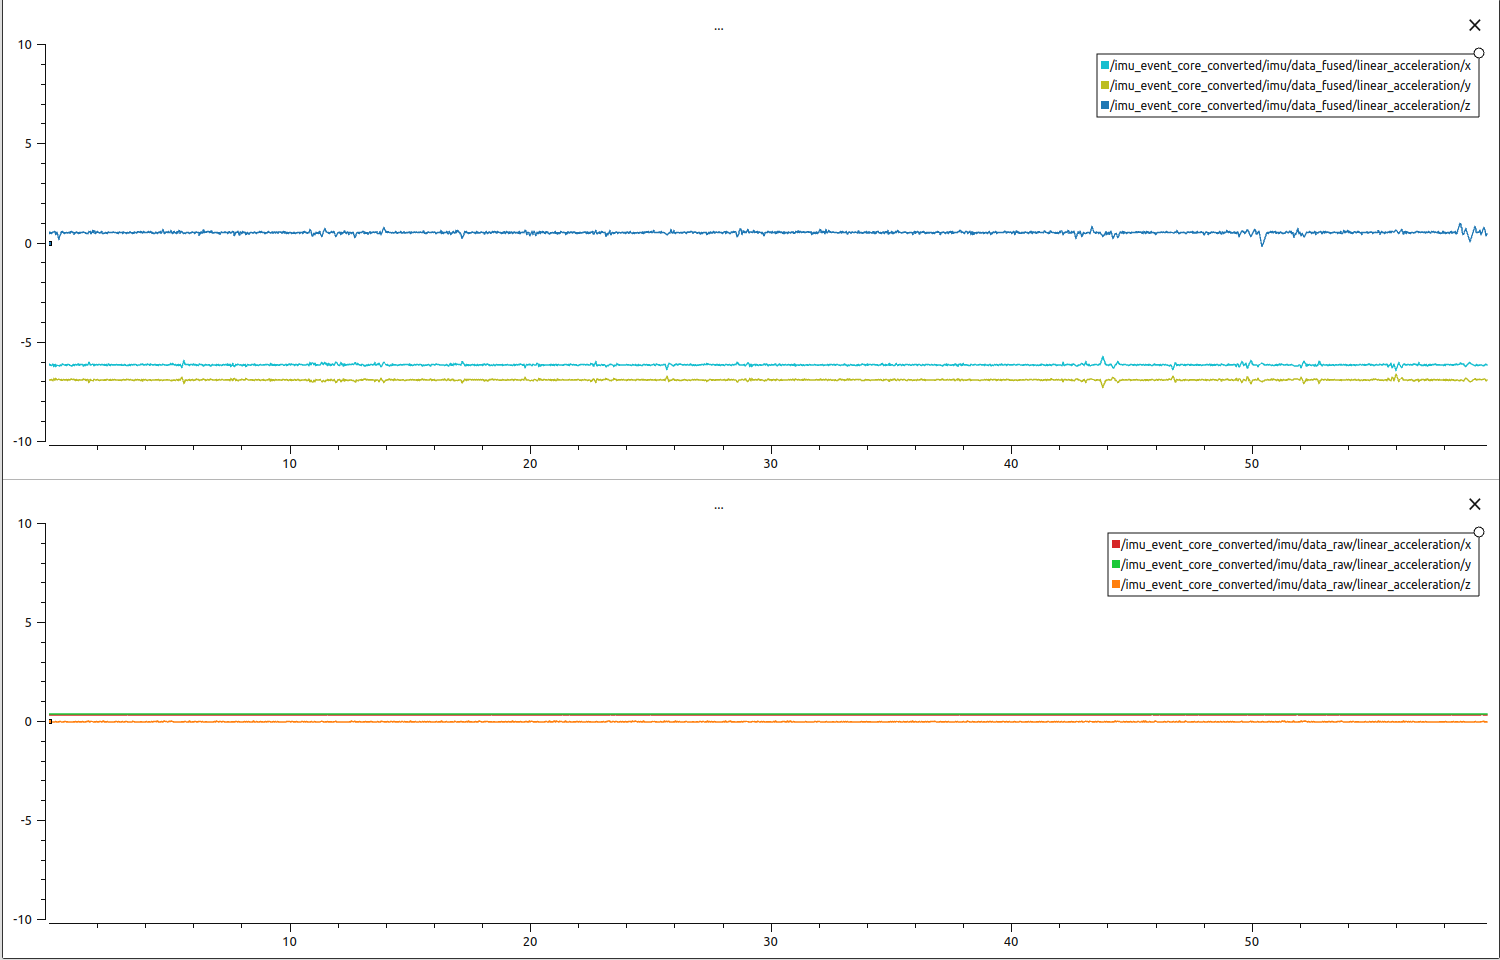
\includegraphics[width=1\columnwidth]{Bachelorarbeit/images/RemovalOfGravity.png}
    \caption{MPU-6050: Madgwick Filter ohne(oben) und mit(unten) Entfernung der Erdanziehungskraft}
    \label{fig:RemovalOfGravity}
\end{figure}
Mit dem Parameter \lstinline{remove_gravity_vector} ist der Filter in der Lage die Erdanziehungskraft aus der linearen Beschleunigung ungefähr auszurechnen und zu stabilisieren. 
\newpage
Nach Anwendung des Filters können somit auch die relativen Orientierungsdaten ermittelt werden.

\begin{figure}[h]
	\centering
    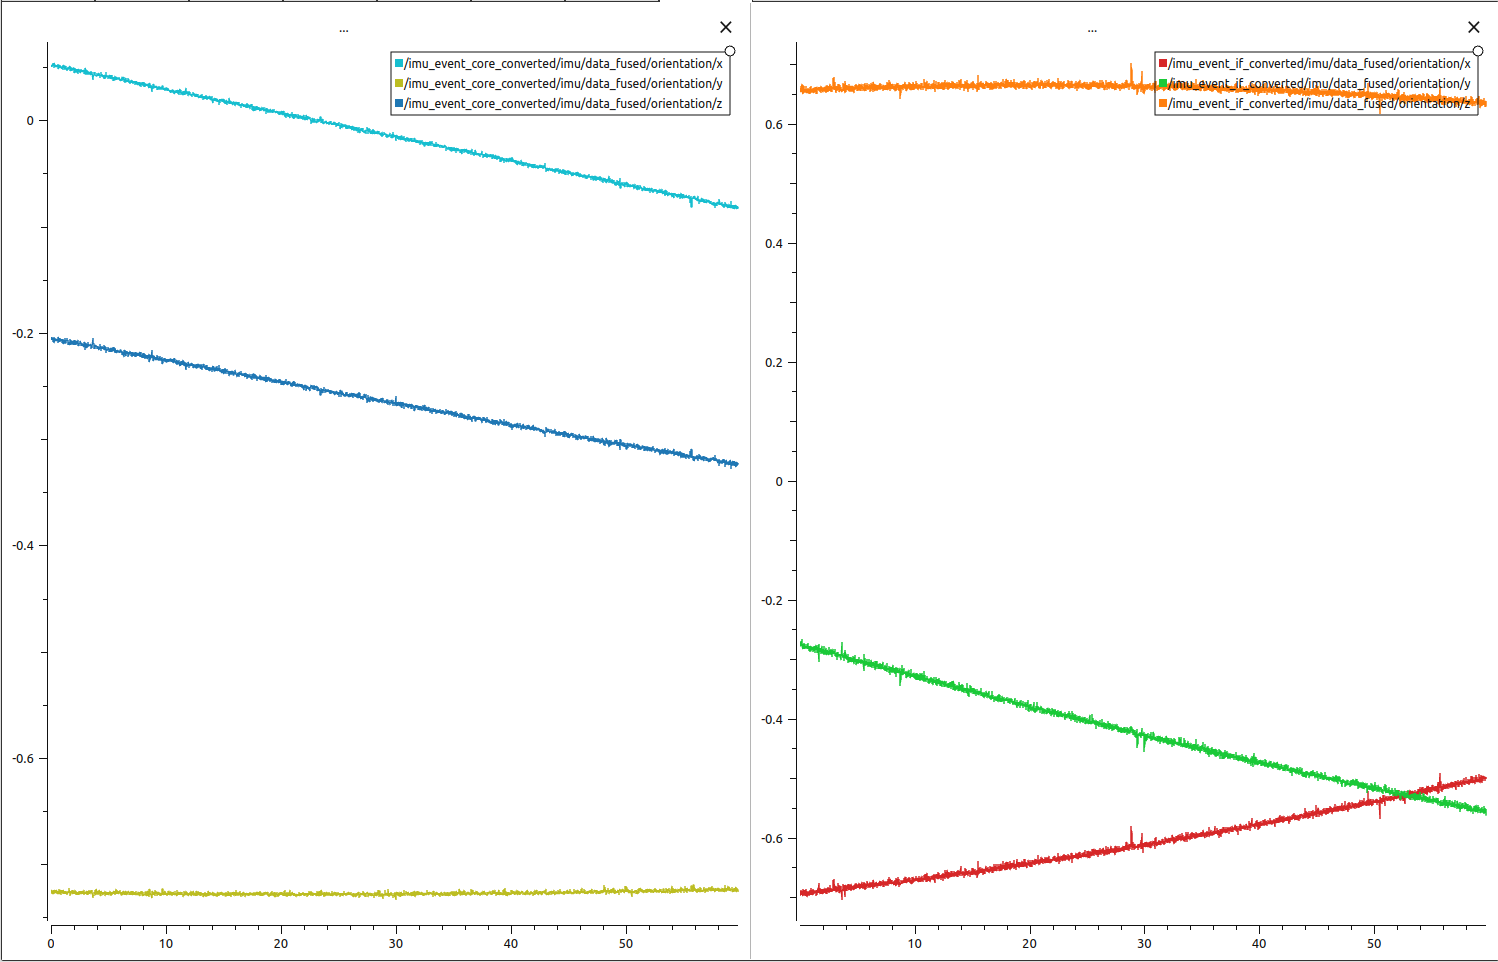
\includegraphics[width=1\columnwidth]{Bachelorarbeit/images/6050-Orientierung.png}
    \caption{Orientierungsdaten des MPU-9250(links) und MPU-6050(rechts)}
    \label{fig:Orientation6050}
\end{figure}
Dabei ist erkenntlich das die Kalibrierung noch nicht optimiert ist und nach einer Weile im Raum driftet, dafür werden jedoch rauschfreie Werte ausgerechnet. 

\newpage
\begin{figure}[h]
	\centering
    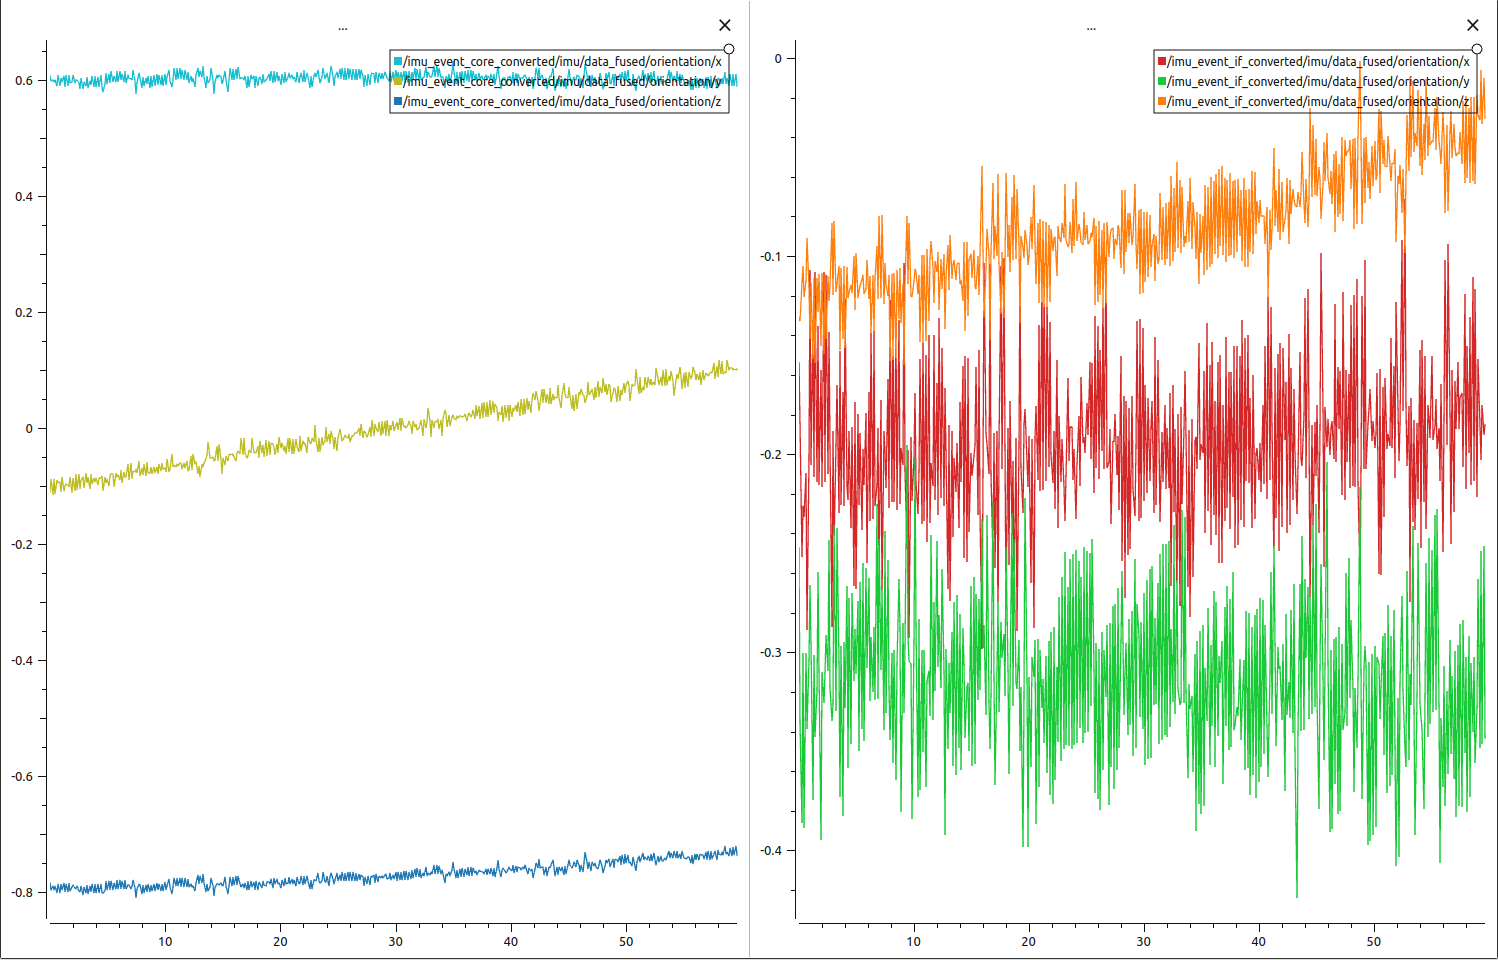
\includegraphics[width=1\columnwidth]{Bachelorarbeit/images/160Orientierung.png}
    \caption{Orientierungsdaten des MPU-9250(links) und MPU-6050(rechts)}
    \label{fig:Orientation160}
\end{figure}
Der BMI160 berrechnet durch die niedrige Datenrate sehr unruhige und auch driftende Werte im Raum. Dieses war durch die langsame Datenrate \ref{fig:RawData160} vorherzusehen, denn für die Ermittelung können schon langsame Schwingungsbewegung zu einer Fälschung der Orientierung führen, hier wurde der Sensor nicht bewegt und trotzdem sind die Daten mit viel Rauschen erkenntlich.

\newpage
Die MPU-9250 Orientierungsberechnung ohne und mit Verwendung des Magnetometerwertes zeigt deutliche Unterschiede der Orientierung.

\begin{figure}[h]
	\centering
    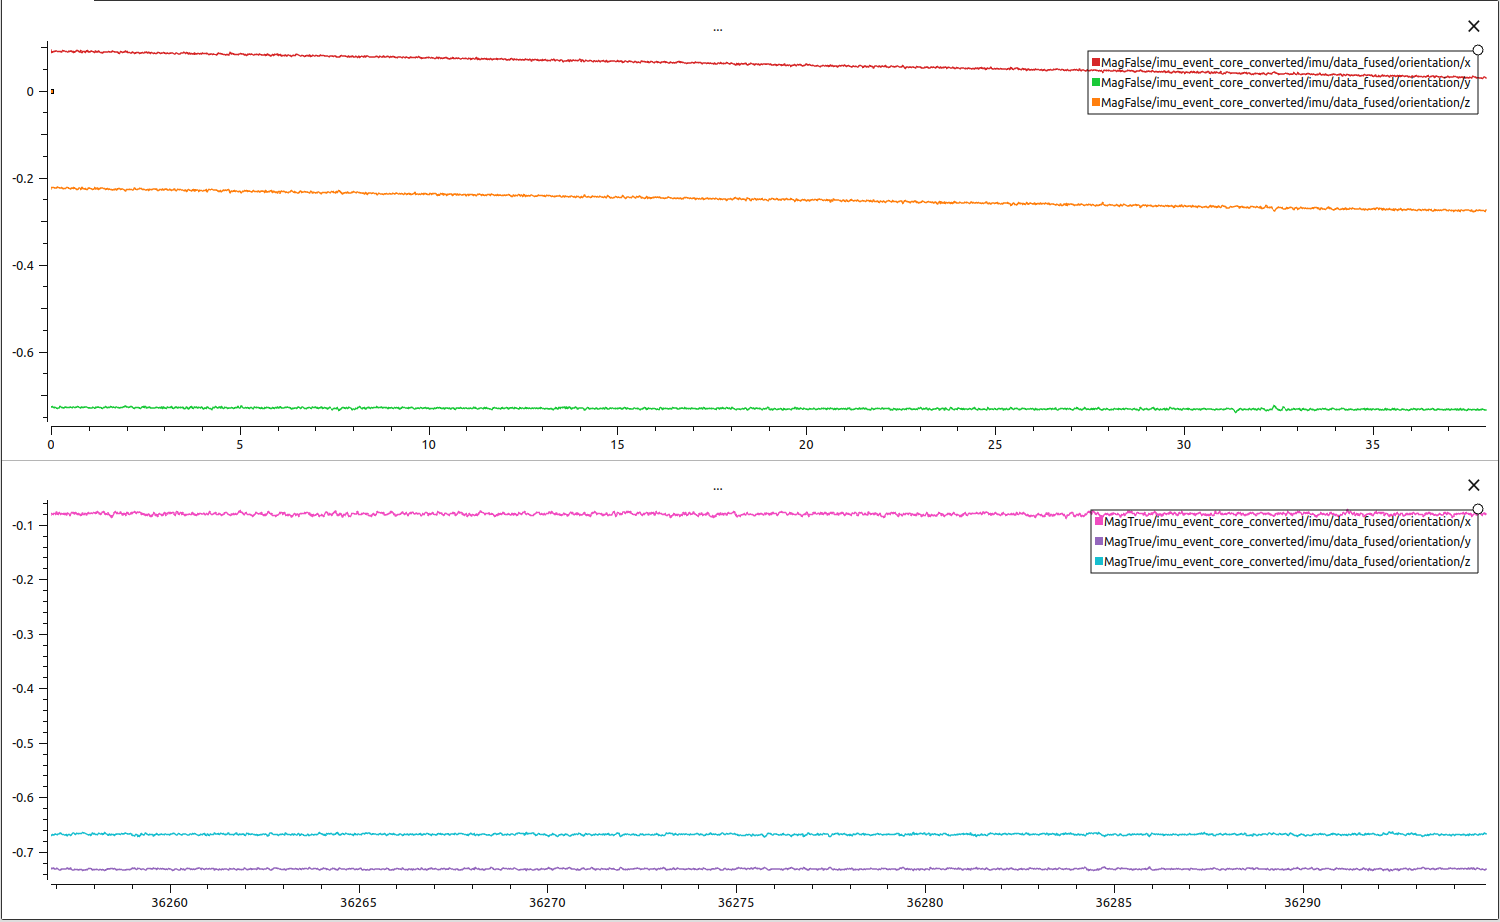
\includegraphics[width=1\columnwidth]{Bachelorarbeit/images/ComparisonMagValueSetTrueAndFalse.png}
    \caption{Vergleich der Orientierung beim einsetzen und ohne das einsetzen der Magnetometerwert}
    \label{fig:MagTrueAndFalse}
\end{figure}
Die Werte driften stärker ab, wenn die Magnetometerwerte nicht mit verwendet werden. Dieses zeigt eine gute Stabilität und genauere Orientierung mithilfe der Kompassdaten. 